\input{./._relpath-to-latexroot.ltx}
\documentclass[\latexroot/\projectname]{subfiles}
\input{\latexroot/@resources/subfile-setup.ltx}

\begin{document}
\whenstandalone{%
  \graphicspath{{../Figures/Cagetti2005tk/}{../images/}}%
}%
\whenintegrated{%
  \graphicspath{{./Figures/Cagetti2005tk/}{./images/}}%
}%

\FloatBarrier
\section{Reproduction Results and Discussion}
\whenintegrated{\label{sec:comparing}}

This section compares the notebook results with the benchmark results in Cagetti and De Nardi (2006). The comparison has to be careful because my notebook solves a fixed-price household problem and uses a young-only stationary distribution diagnostic. The original paper solves a full stationary general equilibrium with young and old households, bequests, market clearing, and calibration to data moments. Therefore, I treat the notebook results as a partial reproduction of the theory mechanism, not as a full replication of the quantitative tables.

\subsection{Convergence and Computation}

The first result is that the value-function iteration now converges. Figure~\ref{fig:convergence} shows the total update norm and the separate update norms for the main value functions. The notebook reaches the stopping rule after 115 iterations, with a final sum norm of $4.78\times 10^{-4}$ against a tolerance of $5.0\times 10^{-4}$. This is important because the later occupational-choice and distribution results are based on a converged fixed-price solution rather than on an unfinished iterate.

\begin{figure}[htbp]
  \centering
  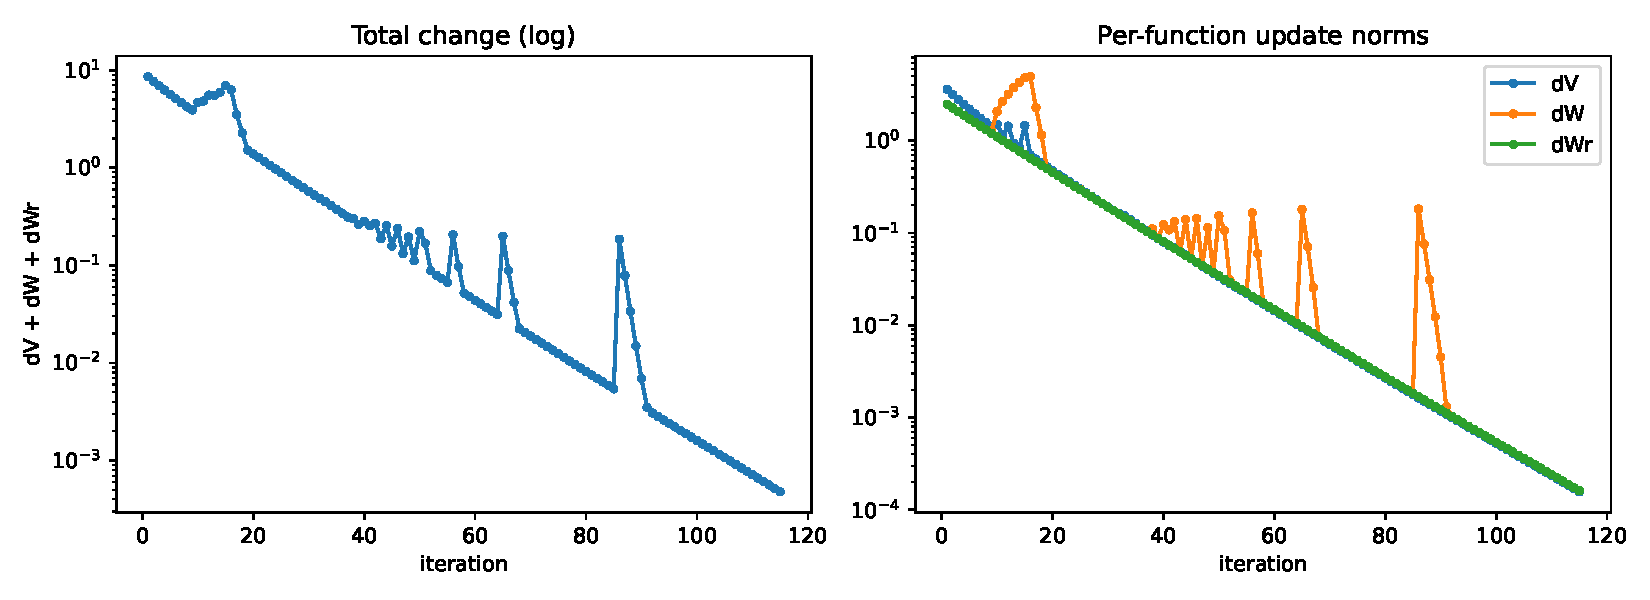
\includegraphics[width=0.86\textwidth]{convergence}
  \caption{Convergence diagnostics for the fixed-price household problem.}
  \whenintegrated{\label{fig:convergence}}
\end{figure}

The enforcement constraint is active in the computation. In the baseline run, all entrepreneurial candidate points are feasible in the resource sense, but only about 12.9 percent of young entrepreneur candidates pass the repayment-versus-default check. For old entrepreneurs the enforcement pass rate is about 67.0 percent. This difference is economically sensible: old high-ability entrepreneurs in the solved grid have a stronger incentive to continue operating firms, while many young households still find the worker branch more attractive.

\subsection{Value Functions and Policy Functions}

Figure~\ref{fig:values-policies-kstar} summarizes the most useful model objects from the notebook. The top-left panel compares the young worker value $V_w$ and young entrepreneur value $V_e$ for high entrepreneurial ability and middle labor productivity. The entrepreneur value is very low at the borrowing-constrained end of the grid, which reflects the difficulty of running a firm with too little collateral. At higher assets, the occupational envelope becomes much closer, and the branch choice is determined by the comparison between the worker outside option and entrepreneurial returns.

\begin{figure}[htbp]
  \centering
  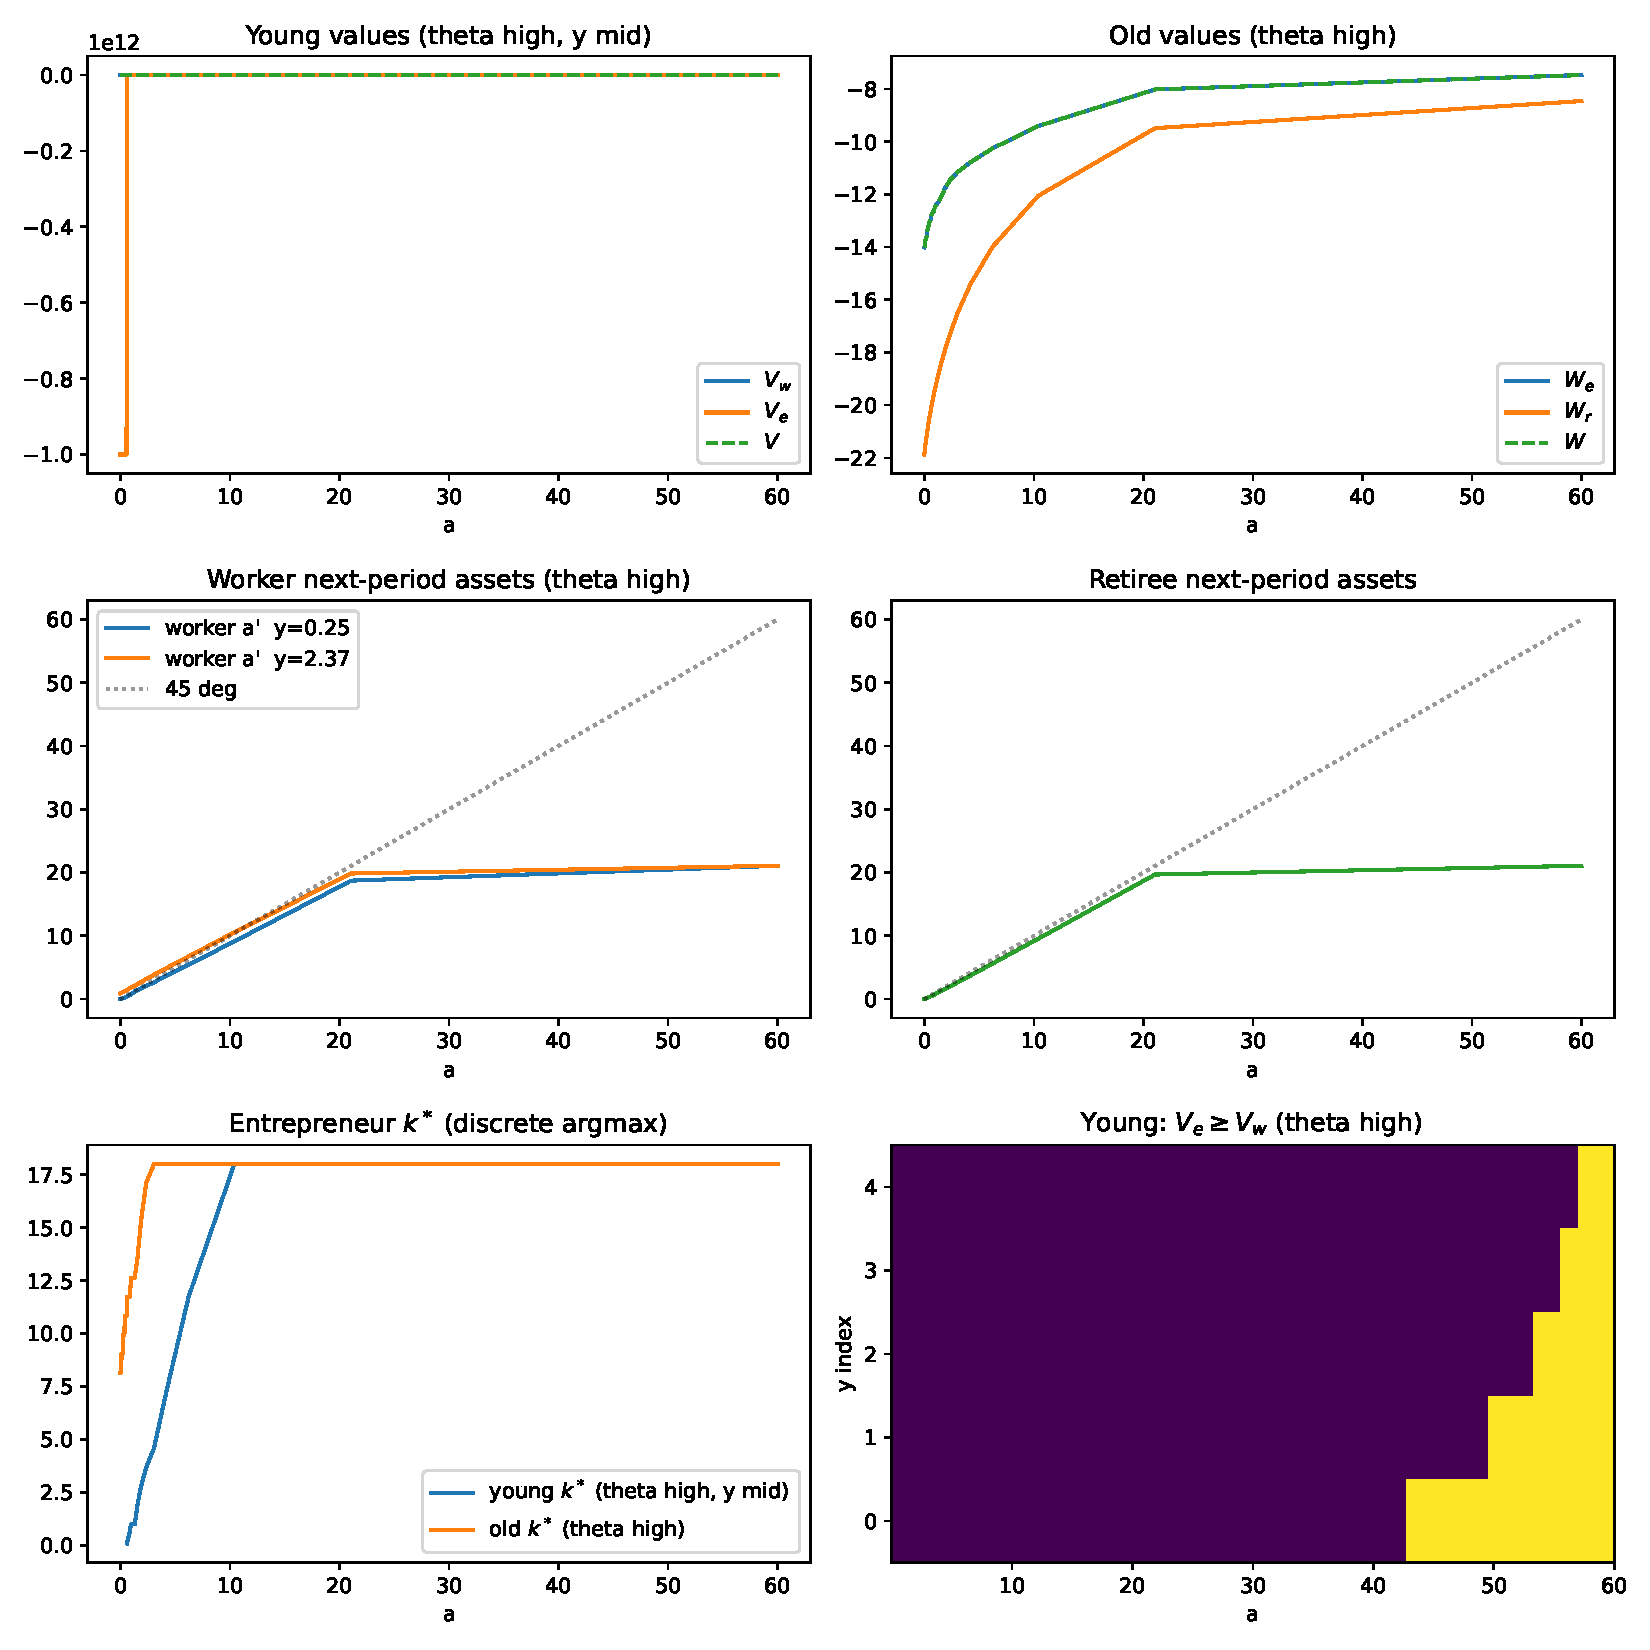
\includegraphics[width=0.92\textwidth]{values_policies_kstar}
  \caption{Value functions, saving policies, occupational choice, and entrepreneurial investment from the notebook.}
  \whenintegrated{\label{fig:values-policies-kstar}}
\end{figure}

The top-right panel shows that old high-ability entrepreneurs prefer continuing entrepreneurship over retirement throughout the plotted asset grid. This matches the intuition of the original paper: once a high-ability entrepreneur has access to the business technology, continuing can be valuable because entrepreneurial returns are high relative to the safe return.

The middle panels show next-period asset policies for workers and retirees. Both policies are below the 45-degree line at high assets in the plotted range, which means households do not keep increasing assets one-for-one forever. This is partly due to the finite grid and fixed-price setting. The bottom-left panel shows the entrepreneurial capital choice $k^\star$. The old entrepreneur reaches a high business scale more quickly, while the young entrepreneur's $k^\star$ rises with assets and then flattens near the upper part of the discrete $k$ grid. This is exactly the mechanism I wanted the reproduction to show: assets relax the ability to operate a larger firm, but the enforcement constraint and the discrete capital grid limit the feasible scale.

The bottom-right panel is the clearest occupational-choice picture. With zero entrepreneurial ability, nobody chooses entrepreneurship. With high entrepreneurial ability, the probability of choosing entrepreneurship is higher for lower labor productivity states and higher assets. In the current run, the share of the asset grid where $V_e\geq V_w$ is 28.7 percent for the lowest labor productivity state and 5.0 percent for the highest labor productivity state. This makes economic sense because high labor productivity raises the worker outside option.

\subsection{Comparison with the Original Paper}

Table~\ref{tab:paper-vs-reproduction} compares the notebook's main numerical outputs with the original paper's benchmark model results. The entrepreneur share is the closest comparison. The original paper reports 7.5 percent entrepreneurs in the baseline model, and the notebook's young-only distribution gives 8.25 percent. This is close enough to show that the occupational-choice mechanism is working in the right range.

\begin{table}[htbp]
  \centering
  \caption{Benchmark Results and Current Reproduction Outputs}
  \whenintegrated{\label{tab:paper-vs-reproduction}}
  \begin{tabular}{p{0.23\textwidth}p{0.18\textwidth}p{0.18\textwidth}p{0.31\textwidth}}
    \hline\hline
    Moment & Original paper baseline & Notebook output & Interpretation \\
    \hline
    Entrepreneur share & 7.50\% & 8.25\% & Close in the fixed-price, young-only diagnostic \\
    Wealth Gini & 0.80 & 0.62 & Too low because full demographic wealth accumulation is not reproduced \\
    Top 1\% wealth share & 31\% & 6.10\% & Far below paper; upper tail is missing \\
    Top 5\% wealth share & 60\% & 27.78\% & Below paper; young-only kernel understates concentration \\
    Capital-output ratio & 3.0 & Not reproduced & Requires general equilibrium aggregation \\
    \hline
  \end{tabular}
\end{table}

The comparison shows both success and limitation. The success is that the notebook reproduces the branch structure well enough to generate an entrepreneur share near the paper's baseline. It also reproduces the qualitative occupational-choice logic: high entrepreneurial ability and sufficient assets make entrepreneurship more attractive, while high labor income makes wage work more attractive.

The limitation is the wealth distribution. The notebook's wealth Gini is 0.62 and its top 1 percent wealth share is only 6.1 percent, far below the paper's baseline values. I do not interpret this as evidence against the original model. Instead, it reflects the narrower reproduction. The original paper's wealth concentration comes from the full distribution over ages, entrepreneurs, retirees, and dynasties, combined with general equilibrium and calibration. My notebook uses only a young-only diagnostic distribution, so it does not yet include the full bequest and old-age wealth accumulation channels that are important for the upper tail.

\subsection{Stationary Distribution Diagnostic}

Figure~\ref{fig:mu-marginal-assets} reports the young-only distribution diagnostic. The right panel shows that the distribution iteration itself converges smoothly. The left panel shows mass both near zero assets and near the upper part of the grid. This tells me that the policy rules are moving households through the asset grid in a stable way. However, it also shows why the distribution comparison is limited. The diagnostic distribution is shaped by the truncated asset grid and does not include the full demographic status dimension, so it cannot fully reproduce the paper's top wealth shares.

\begin{figure}[htbp]
  \centering
  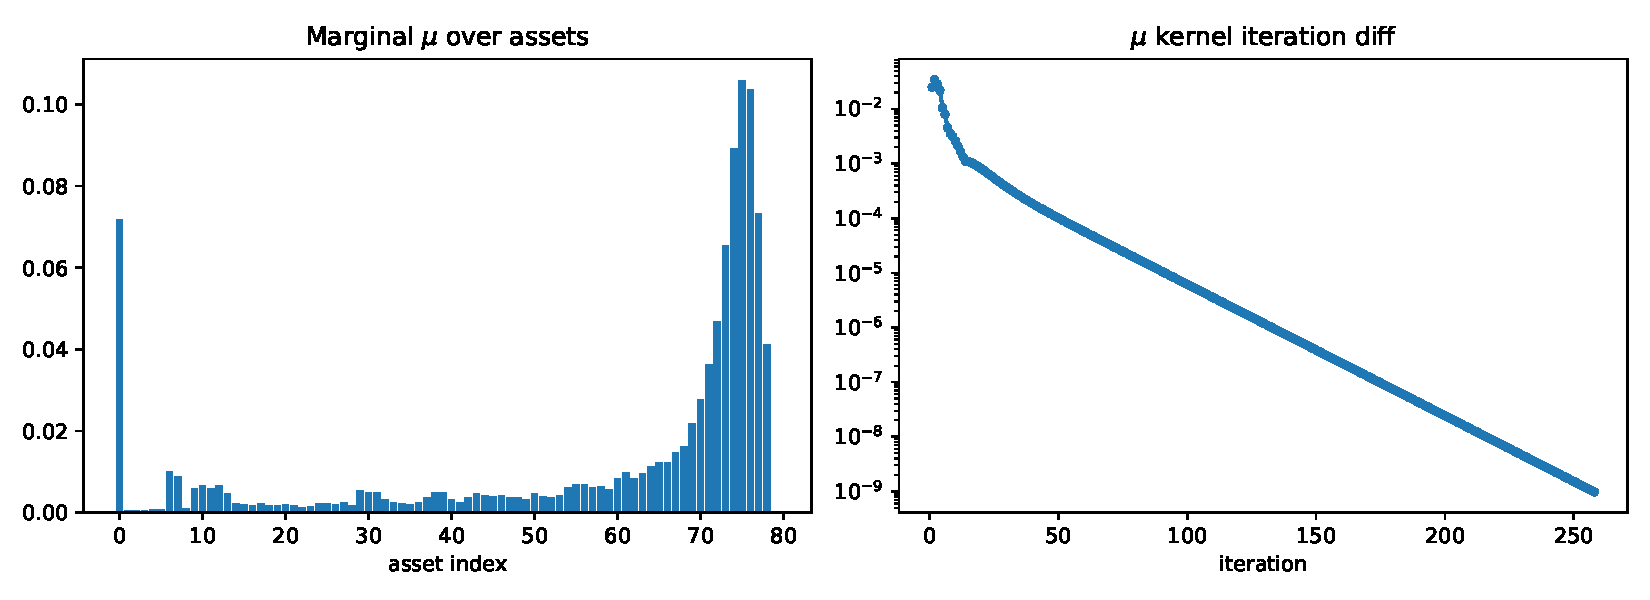
\includegraphics[width=0.86\textwidth]{mu_marginal_assets}
  \caption{Young-only asset distribution diagnostic from the notebook.}
  \whenintegrated{\label{fig:mu-marginal-assets}}
\end{figure}

The partial-equilibrium counterfactuals in the notebook should also be read cautiously. Some one-at-a-time changes, such as raising the interest rate to 7.5 percent or changing the pension share, converge and leave the middle-productivity young entrepreneurship region close to the baseline. Other changes, such as shutting down the bequest motive or increasing high entrepreneurial ability, do not converge within the shortened counterfactual iteration cap. I therefore use these rows only as diagnostics, not as reproduced versions of the paper's counterfactual tables.

Overall, the reproduction is strongest on the household problem and weaker on the aggregate distribution. It succeeds at organizing the model, solving the baseline fixed-price problem, and showing the occupational-choice mechanism. It does not yet reproduce the full wealth-concentration result, because that requires the full stationary equilibrium and demographic distribution.

\smartbib

\end{document}
